\chapter{Radionuclide therapy and dosimetry}

\section{Introduction}
%%%%%%%%%%%%%%%%%%%%%%
In nuclear medicine, radiopharmaca are mostly used for diagnostic
imaging (with SPECT or PET) and activity concentration measurements in
samples (with a gamma counter). For that purpose, the radiopharmacon is
labeled with a single photon or a positron emitting isotope. The
photon energy of the single photon emitter is ideally between 100 and
200 keV, because that is a good compromise between good penetration of
human tissues and good stopping by detector crystal. This is one of
the reasons why \textsuperscript{99m}Tc\ (emitting photons of 140 keV) is the most used
radionuclide for single photon emission imaging. Positron emission will
always produce 511 keV photons. That is a bit higher that we would
have liked; for PET, there was no choice but to design detectors with
sufficient stopping power. Ideally, the isotope would emit nothing
else, because other emitted particles will not contribute to imaging,
but they will damage the tissues (DNA) they traverse.

In recent years, radionuclide therapy is being used increasingly in
cancer therapy. Radionuclide therapy makes use of molecules or other
particles that accumulate preferentially in tumors, and which are
labeled with radioactive isotopes (radionuclides). The aim is that
this radiation will destroy the tumor, with minimal damage to the
surrounding healthy tissues. For that purpose, the radiation should
have a small penetration depth, as is the case for electrons (aka
$\beta^-$), protons and $\alpha$-particles (particle consisting of two
protons and two neutrons, He$^{2+}$). Table \ref{tab:rntisotopes} and
figure \ref{fig:223Ra} list the main emissions by a few of such
radionuclides. The decay scheme of $^{223}$Ra is complex, because several
of its daughter products are radiactive as well.

Most radionuclides used for therapy not only emit $\beta$ or $\alpha$
particles, but also photons. The drawback of these photons is that
they cause some radiation to the healthy tissues, but an advantage is
that images can be made of the distribution of the radionuclide,
enabling accurate dose verification (at least if the photon energies
are suitable for imaging).

If the radiopharmacon has high affinity for the tumor and is very
specific, i.e. it binds to the tumor and to (almost) nothing else,
then the therapy can be more effective than external beam therapy for
two reasons: it will treat all metastases, even small ones that may
not be revealed by imaging, and a high radiation can be achieved with
minimum damage to the surrounding healthy tissues.

To be effective, the amount of radioactivity administered to the
patient should be high enough to destroy the tumors, but at the same
time low enough to ensure that the radiation to healthy tissues (which
may also accumulate some of the radioactivity) remains below safety
limits. Consequently, it is important to estimate the expected dose
distributions before treatment, and determine the delivered doses
after treatment.

%------------------
\begin{table}[h]
  \centering
  \caption{Some radionuclides used in radionuclide therapy} 
  \label{tab:rntisotopes}
  %------------------
  %% \vspace{2mm}
  %% \begin{tabular}{|c c c|}
  %%   % Hindorf, C., Chittenden, S., Aksnes, A. K., Parker, C., & Flux,
  %%   % G. D. (2012). Quantitative imaging of 223Ra-chloride
  %%   % (Alpharadin) for targeted alpha-emitting radionuclide therapy of
  %%   % bone metastases. Nuclear medicine communications, 33(7),
  %%   % 726-732. DOI:10.1097/MNM.0b013e328353bb6e
  %%   % 
  %%   \hline
  %%   {\bf $^{223}$Ra} &  half-life & 11.44 days    \\
  %%   \hline
  %%   emission          & mean energy & intensity\\
  %%                     &   keV         &    \% \\
  %%   \hline
  %%   $\alpha$          & $26.4 \cdot 10^3$  &  100  \\
  %%   $\beta^-, \gamma$ & $1.4 \cdot 10^3$ & 100 \\
  %%   \hline
  %%             &  12    & 22.9 \\
  %%             &  81.1  & 15.2 \\
  %%             &  83.8  & 25.1 \\
  %%             &  95    & 11.5 \\
  %%    $\gamma$ &  122   &  1.2 \\
  %%             &  144   &  3.3 \\
  %%             &  154   &  5.7 \\
  %%             &  270   & 13.9 \\
  %%             &  324   &  4.0 \\
  %%             &  338   &  2.8 \\
  %%   \hline
  %% \end{tabular}
  %------------------
  \vspace{2mm}
  \begin{tabular}{|c c c|}
    \hline
    {\bf $^{131}$I} &  half-life    &  8.03 days\\
    \hline
    emission & mean energy & intensity\\
             &   keV         &    \% \\
    \hline
    $\beta^-$ &  182          &  100  \\
    \hline
              &  80   &  2.62 \\
              & 284   &  6.12 \\
    $\gamma$ & 364   &  81.5 \\
             & 637   &  7.16 \\
             & 723   &  1.77 \\
    \hline
  \end{tabular}
  \vspace{2mm}
  %------------------
  %\centering
  %\caption{}
  \begin{minipage}{0.45\textwidth}
  \vspace{2mm}
  \begin{tabular}{|c c c|}
    \hline
    {\bf $^{177}$Lu} &  half-life    & 6.6 days \\
    \hline
    emission & mean energy & intensity\\
             &   keV         &    \% \\
    \hline
    $\beta^-$ &  133         & 100   \\
    \hline
    X-ray    &  55  &   4.28 \\
    $\gamma$ &  113 &   6.23 \\
             &  208 &  10.41 \\
    \hline
  \end{tabular}
  %------------------
  \vspace{2mm}
  \begin{tabular}{|c c c|}
    \hline
    {\bf $^{90}$Y } &  half-life    &  64.1 h\\
    \hline
    emission & mean energy & intensity\\
             &   keV         &    \% \\
    \hline
    $\beta^-$ &   933.6      & 100   \\
    $\beta^+$ &  ($^{90}$Zr 0+ decay)  & 0.0032   \\
    \hline
     $\gamma$ &    &   \\
    \hline
  \end{tabular}
  \end{minipage}\\
  %% 90Y normally decays to the 90Zr ground state, it has a minor
  %% branch for decaying to the 0+ first excited state of 90Zr. 
  %% 0+ means spin 0 and even parity. The 90Zr decay is from the 0+ first
  %% excited state (1.76 MeV) to the 0+ ground state.
%------------------
\end{table}

\begin{figure}[htb]
  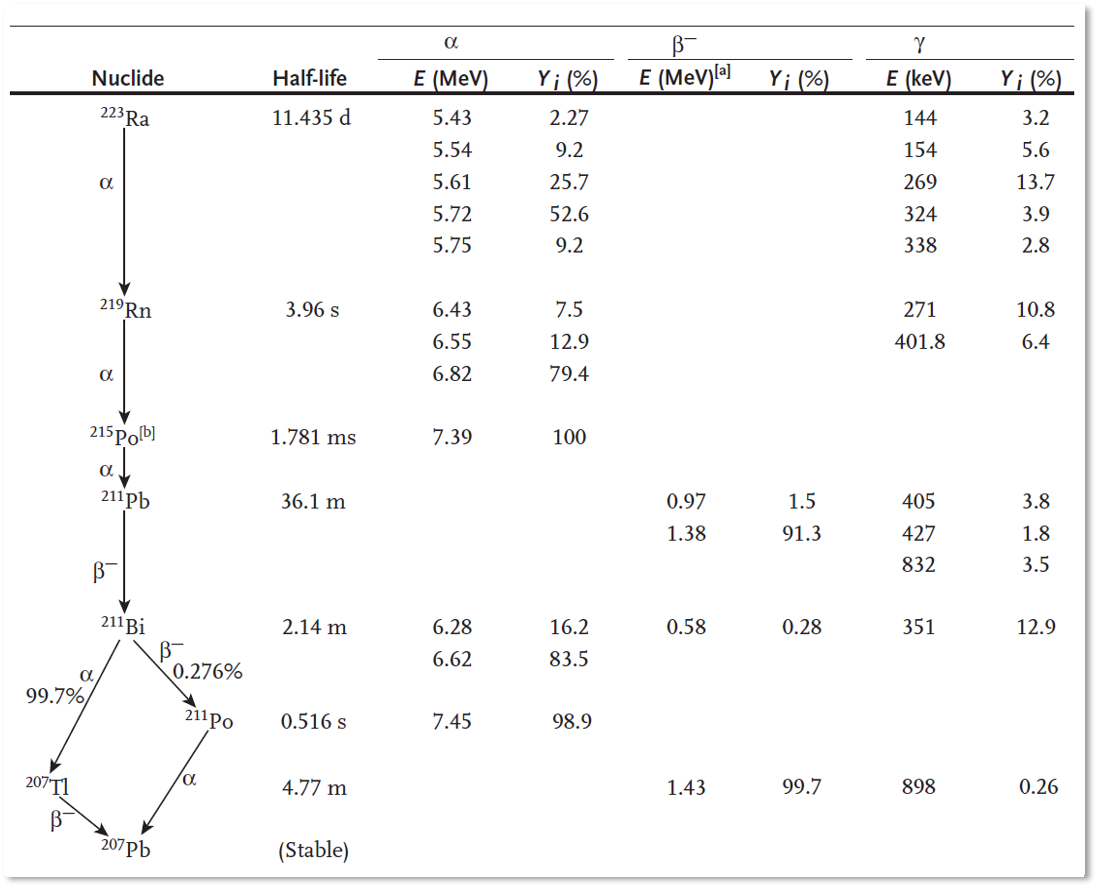
\includegraphics[width=\textwidth]{figs/fig_223Ra.png}
  \centering
  \caption{\label{fig:223Ra} \emph{Decay scheme of \, $^{223}$Ra,
      based on \cite{Martin2006}.}}
\end{figure}


\section{MIRD formalism}
%%%%%%%%%%%%%%%%%%%%%%%%
MIRD refers to the Committee on Medical Internal Radiation Dose of the
Society of Nuclear Medicine, which provides standard methods for
internal radiation dosimetry. The focus has mostly been on producing
reasonable dose estimates, to assess and control the risk associated
with diagnostic imaging. These days, refinements are being made for
more accurate dose calculations as required for radionuclide therapy.

The basic principles of internal dosimetry have already been explained
in chapter \ref{chap:biol}. MIRD uses the same principles, but
formulates them slightly differently, introducing the dose rate and
the S-factors. Another difference is that in chapter \ref{chap:biol},
we integrated the activity over time to compute the total number of
decays, and then computed the resulting dose from them. MIRD computes
the dose associated with a single decay event (the dose rate), and
integrates that over time.

The body of the patient is considered as a collection of 3D regions
which contain an amount of radioactivity. To compute the dose (in Gy)
received by a particular region, that region is treated as the {\em
  target region} $r_T$, while all regions (including $r_T$) are
considered one by one as {\em source regions} $r_S$. The source region
contains a time dependent activity $A(t)$, which is usually assumed
uniform for convenience. At each point in time, that activity $A(t)$
in the source region produces a dose rate $\dot{D}(t)$ in the target
region. It is assumed that the two are proportional:
\begin{equation}
 \frac{d D(t)}{dt} = \dot{D}(t) = S \; A(t) \label{eq:doserate}
\end{equation}
The activity $A(t)$ is expressed in Bq, the dose rate $\dot{D}(t)$ in
Gy/s. Consequently, the unit of $S$ is Gy~/~(Bq~s) = Gy.

The factor $S$, usually called the S-value, accounts for the
following:
\begin{itemize}
  \item the probability that a particular particle ($\gamma, \beta^+,
    \beta^-, \alpha$, \ldots) is produced during a decay in source
    region $r_S$,
  \item the energy of each particle,
  \item the probability that the particle reaches target region $r_T$,
  \item the probability that it deposits (part of) its energy in
    $r_T$,
  \item the mass of $r_T$.
\end{itemize}
Because patients breathe, the shape of $r_S$ and $r_T$ and the
distance between them may change, which would affect
$S$. Consequently, $S$ is a function of time, although that is
typically ignored to keep the problem tractable. The S-value can be
written as
\begin{equation}
  S(r_T \leftarrow r_S, t) = \frac{1}{M(r_T,t)}
     \sum_i p_i \; E_i \; \phi(r_T \leftarrow r_S, E_i, t)
  \label{eq:Svalue}
\end{equation}
$M(r_T,t)$ is the mass of $r_T$, which might be time dependent. The
summation is over all emissions $i$ that may occur during a decay;
$p_i$ is the branching ratio, i.e. the probability that emission $i$
will occur during a decay. $E_i$ is the energy of particle $i$ and
$\phi(r_T \leftarrow r_S, E_i, t)$ gives the fraction of the energy
that this particle is expected to deposit in $r_T$. Thus, $\phi$
depends on the geometry and attenuation of $r_T$ and $r_S$ and the
structures between and around them.

Since the dose rate in $r_T$ depends on all the radioactivity inside the
patient's body, we have to sum over all $r_S$:
\begin{equation}
  \dot{D}(r_T, t) = \sum_j S\left(r_T \leftarrow r_{S_j}, t\right)
                \; A\left(r_{S_j}, t\right)
\end{equation}
The dose in $r_T$ is obtained by integrating over time:
\begin{align}
  D(r_T) &= \int_0^{T_D} \dot{D}(r_T, t)\;dt \nonumber\\
     &\simeq \sum_j S\left(r_T \leftarrow r_{S_j} \right)
        \int_0^{T_D} A\left(r_{S_j},t\right) dt \nonumber\\
     &= \sum_j S\left(r_T \leftarrow r_{S_j} \right)
        \tilde A \left(r_{S_j} \right) \label{eq:mirddose}
\end{align}
$T_D$ is some interesting time duration. In many cases, one can set
$T_D = \infty$, because the effective half life (combining decay half
life and the biogical dynamics) of the radionuclide will be
short. $\tilde A$ is the time integrated activity. To put $S$ in front
of the integral sign, we had to make the common approximation that it
does not depend on time.

The time integrated activity $\tilde A$ has no units, since Bq is
the number of desintegrations per s, and a number is unitless. In
practice, one often normalizes $\tilde A$ with the administered
activity $A_0$:
\begin{equation}
  \tilde a(r_S) = \frac{\tilde A(r_S)}{A_0}
\end{equation}
and therefore $\tilde A(r_S) = \tilde a(r_S) A_0$. The unit of $\tilde
a$ is time, and for that reason it was called the {\em residence
  time}. If all the administered activity $A_0$ would stay for a short
duration $\tilde a(r_S)$ in the region $r_S$ and then vanish, then the
same $\tilde A(r_S)$ would be obtained. Since 2009,
$\tilde a(r_S)$ is
called the {\em time-integrated activity coefficient} of $r_S$
\footnote{In 2009, the MIRD committee adopted a standardization of
  nomenclature (Journal of Nuclear Medicine, 2009; 50: 477-484).}.

To apply equation (\ref{eq:mirddose}) for treatment planning or
verification, we need
\begin{enumerate}
\item a 3D segmentation (delineation) of all important structures:
  organs, parts of organs, tumors, lesions, \ldots, to produce the set
  of regions
\item the function $\phi(r_T \leftarrow r_S, E_i, t)$ for all possible
  region pairs ($r_S$, $r_T$), all relevant particles $i$ and all
  relevant energies $E_i$.
\item the activity $A\left(r_{S_j},t\right)$ as a function of time in
  all these regions,
\end{enumerate}
%
This should really be done for each individual patient (``personalized
dosimetry''). Because that is very difficult, the segmentation and
calculation of $\phi(r_T \leftarrow r_S, E_i, t)$ have first been
addressed based on models of ``average patients''. Figure
\ref{fig:MIRD} shows two such models, an early one based on simplified
shapes and a more recent and realistic model using non-uniform
rotational B-splines (NURBS). Similar models have been developed for
children of different ages.
%
\begin{figure}[htb]
  \centering
 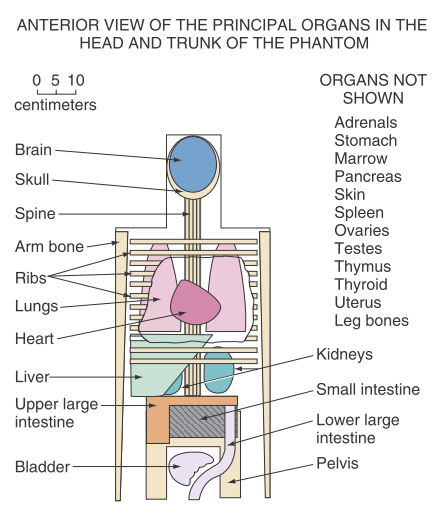
\includegraphics[bb=0 0 250 300,width=0.49\textwidth]{figs/fig_MIRD_average_man.png}
 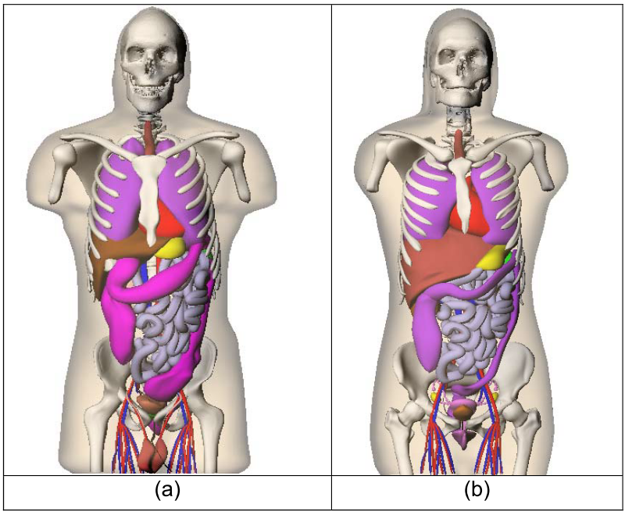
\includegraphics[bb=0 0 300 300,width=0.5\textwidth]{figs/fig_NURBS_Segars.png}
\caption{\label{fig:MIRD}
  \emph{Left: representation of the average man for MIRD dose
    computation, as used in 1969 \cite{Cherry}. Right: human body
    models based on non-uniform rational B-splines (NURBS)
    \cite{Stabin2008}.}}
\end{figure}

When the patient model is available, the S-value can be computed with
equation (\ref{eq:Svalue}) for every region pair and for all
radionuclides of interest. For electrons, positrons and
$\alpha$-particles, one can usually assume that their energy is
deposited locally. That makes the calculation of $\phi(r_T \leftarrow
r_S, E_i, t)$ very easy:
\begin{itemize}
\item if $r_S \neq r_T$, then $\phi(r_T \leftarrow r_S, E_i, t) \simeq 0$
\item for $r_S = r_T$: $\phi(r_S \leftarrow r_S, E_i, t) \simeq 1$
\end{itemize}
On the other hand, for photons the calculations are very complicated
and have to be done with Monte Carlo simulation.

Finally, to obtain a dose for a particular case, we need to determine
the time-activity curves $A\left(r_{S_j},t\right)$ for each organ
$r_{S_j}$. Currently, this is done by acquiring SPECT or PET scans and
manually segmenting the organs in the activity images, or in the
corresponding CT images (relying on the spatial alignment produced by
the SPECT/CT or PET/CT system). The time-activity curve is typically
obtained by acquiring a dynamic SPECT or PET scan. For tracers with
long (physical and biological) half life, some additional scans at
later time points may be required. A good balance must be found
between minimizing the number of scans (and their duration) for
optimal patient comfort, and obtaining sufficient samples to reach an
acceptable accuracy. In single photon emission imaging, some of the
SPECT or SPECT/CT scans may be replaced by planar imaging to improve
the temporal resolution (early after injection) or to reduce the
imaging time (late after injection).

The anatomical models have been designed for assessing the typical radiation
dose associated with diagnostic procedures. Because these doses are
relatively low, it is assumed that the dose estimates obtained for
such average patients are sufficiently accurate for producing clinical
guidelines on the activity to be injected for different tracers and
imaging tasks. Novel tracers are often first characterized in animal
experiments. If those tests produce good results, they are evaluated
in a small group of healthy volunteers, using one or multiple SPECT/CT
or PET/CT scans, manual organ delineation and the S-values from the
average patient. Because organ delineation is extremely time
consuming, the delineation is usually restricted to source organs that
accumulate a significant amount of activity and target organs that are
known to be radiosensitive. The resulting radiation doses (in mGy or
Gy) can then be converted to an effective dose (in mSv or Sv) by
multiplying the energies with the appropriate quality factor Q (table
\ref{tab:qualfactor}) and computing the weighted sum of the organ
doses \ref{tab:effdose}.

Application of such models to compute the required activity for
radionuclide therapy is controversial, because the model may deviate
strongly from the individual patient. However, because no clinical
tools are currently available for accurate personalized dosimetry,
they are often used for estimating tumor and organ doses in
radionuclide therapy as well. This is likely to change in the next
several years. It is found that ``deep learning'' (using multiple
layers of convolutional neural networks or CNNs) is an excellent tool
to capture the prior knowledge of experts, and it is increasingly
being used for organ segmentation in clinical images. In addition, the
execution time of Monte Carlo simulation can be decreased from several
days to several minutes by implementing them in a clever way on
GPU. Consequently, personalized dosimetry for radionuclide therapy in
clinically acceptable times and with acceptable efforts seems
possible.

\section{Radiation Biologically Effective Dose (BED)}
%%%%%%%%%%%%%%%%%%%%%%%%%%%%%%%%%%%%%%%%%%%%%%%%%%%%
As mentioned above, for diagnostic applications, the effect of the
radiation is converted to an effective dose in mSv using a simple
weighted sum of organ doses. That approach is too simplistic for
application in radionuclide therapy, where the doses are much higher
and errors in dose calculation can result in undertreatment or
irreversible damage to healthy tissues.

In radionuclide therapy, the aim is to destroy the tumor while
minimizing the toxicity to the normal tissues. Therefore, we have to
estimate the biological effects of the radiation on the normal tissues
and the tumor.

Suppose that a piece of tissue, consisting of $N$ cells, is being
irradiated with a particular dose rate $\dot D$. And assume also that
this dose rate kills on average a fraction $k_{\dot D}$ per unit of
time. Then at any time $t$, the expected number of dying cells per
unit of time would equal
\begin{equation}
  \frac{d N(t)}{dt} = - k_{\dot D} N(t)
\end{equation}
After irradiating that tissue for a finite time $T$, the expected
number of surviving cells will be
\begin{equation}
  N(T) = N(0) e^{- k_{\dot D} T}
\end{equation}
%
Assuming that $k_{\dot D}$ can vary as a function of time, this
generalizes to
\begin{equation}
  N(T) = N(0) e^{- \int_0^T k_{\dot D}(t) dt}
\end{equation}
%
If we assume that $k_{\dot D}$ is proportional to the dose rate
$\dot D$, we can write
\begin{equation}
  N(T) = N(0) e^{- \alpha \int_0^T \dot D(t) dt} = N(0) e^{-\alpha
    D(T)}
   = N(0) e^{-\mathrm{BED}}
\end{equation}
where $D(T)$ is the total dose accumulated at time $T$. The exponent
$\alpha D(T)$ is called the {\em Biologically Effective Dose} or {\em
  BED}. The value $\exp(-\mathrm{BED})$ is the fraction of surviving
cells.

However, it has been observed that the BED depends non-linearly on the
dose. This can be explained intuitively as follows. Radiation damages
the tissue mostly by ionizing DNA molecules. It is possible that a
single hit by a photon or electron produces so much damage to a DNA
molecule that the cell dies. But it is also possible (and more
likely) that a single hit produces an error in the DNA that can still
be repaired. However, this sublethal damage could become lethal, if
that same DNA molecule would be hit a second time during the same
treatment. Assuming a sublethal hit is more likely than a lethal one,
and that the probability of hitting the same location more than two
times is very small, the cell killing could be well approximated as
\begin{equation}
  k_{\dot D}(t) = \alpha \dot D(t) + 2 \beta D(t) \dot D(t)
   \label{eq:kdotD}
\end{equation}
The first term corresponds to a single lethal hit at time $t$. The
second corresponds to the lethal combination of two sublethal hits,
one which happened between 0 and $t$, and the second one at time $t$.
%
\footnote{The factor 2 in the second term of (\ref{eq:kdotD}) is added
  to make the final expression (\ref{eq:BED}) slightly shorter. We can
  add any factor, it will be absorbed in $\beta$, which must be
  determined from measurements.}
%
Integration over time produces
\begin{align}
  \mbox{BED} &= \int_0^T k_{\dot D}(t) dt \nonumber\\
  &= \alpha \int_0^T \dot D(t) dt
      + 2 \beta \int_0^T D(t) \dot D(t) dt\nonumber\\
  &= \alpha \int_0^T \frac{dD(t)}{dt} dt
      + 2 \beta \int_0^T D(t)\frac{dD(t)}{dt} dt\nonumber\\
  &= \alpha D(T) + \beta \int_0^T \frac{d D^2(t)}{dt} dt \nonumber\\
  &= \alpha D(T) + \beta D^2(T) \label{eq:BED}
\end{align}

This expression can be further refined to include also the effect of
repair mechanisms. After sublethal damage, the cell may be able to
undo that damage, in which case it would survive a second sublethal
hit. Assume for convenience that the probability of repair is constant
over time, such that a fraction $\mu$ of the damaged cells heal
themselves per unit of time. Then if $M$ cells took a sublethal hit at
time $s$, only $M e^{-\mu (t - s)}$ of them would still be damaged at
time $t > s$. Adjusting equation (\ref{eq:BED}) accordingly produces
\begin{align}
  \mbox{BED} &=\;\; \alpha \int_0^T \dot D(t) dt
  + 2 \beta \int_0^T \dot D(t) dt
  \int_0^t \dot D(s) e^{-\mu(t-s)}ds \nonumber\\
  &=\;\; \alpha D(T) + \beta \, G \, D^2(T) \label{eq:BEDrepair}\\
  \mbox{with\;\;} G &=\;\; \frac{2}{D^2(T)} \int_0^T \dot D(t) dt
    \int_0^t \dot D(s) e^{-\mu(t-s)}ds \nonumber
\end{align}
The G-factor is called the Lea-Catcheside factor (after the authors
who derived these equations). It is easy to check that with $\mu =
0$, i.e. no cell repair, equation (\ref{eq:BEDrepair}) reduces to
(\ref{eq:BED}). Fortunately, normal cells are typically better at
repairing radiation damage than tumor cells.

\section{Dosimetry software}
%%%%%%%%%%%%%%%%%%%%%%%%%%%%
Several software tools have been developed and commercialized to
support dosimetry calculations. The first tools (e.g. Olinda/EXM,
\footnote{Organ Level INternal Dose Assessment \& EXponential
  Modeling} developed by Vanderbilt University, TN, USA and recently
commercialized) focused on dosimetry for diagnostic imaging
procedures. This kind of software takes as input the activity values
in organs at a few different time points, and provides
\begin{itemize}
  \item pre-computed S-values based on anatomical models, such as in
    figure \ref{fig:MIRD} (and listed in MIRD pamphlet 11), for many
    radionuclides, and
  \item software for fitting kinetic models, typically a sum of
    exponentials, which are used to interpolate between the time
    points and extrapolate to infinity in a sensible way.
\end{itemize}
The output is the dose in mGy to all organs, and the corresponding
effective dose in mSv.

Some research teams share their more recent software tools for
personalized internal dosimetry. An example is the LundaDose Program
from Lund University, Sweden. This program focuses on internal
dosimetry for therapy with $^{177}$Lu or $^{90}$Y labeled
molecules. It takes SPECT/CT images as input and computes the organ
and tumor doses with Monte Carlo simulation. Other similar free
software packages can be found at mirdsoft.org, www.idac-dose.org and
www.opendose.org.

By taking directly the images of the activity distribution as input,
the need for segmenting the source organs is eliminated. The Monte
Carlo simulation can make use of the activity in each voxel, or in
other words, each voxel is treated as a source region $r_S$. And
similarly, the dose can be computed in each voxel. This is called {\em
  voxelized dosimetry}. It is not only more convenient, it is also
more accurate, because it eliminates the need for assuming a uniform
activity distribution within large source and target regions. For the
final analysis of the dose images, still organ and lesion segmentation
is necessary for the target regions $r_T$, because we need to know
where the tumor and the radiosensitive organs are. However, the
analysis of the dose in regions $r_T$ can now be made more
informative, by taking into account the non-uniform dose distribution
in the region.

\section{Examples}
%%%%%%%%%%%%%%%%%%
% isotopes 131-I, 177-Lu, 90-Y, 223-Ra
% radiopharmaceuticals
%    - 131I NaI (thyroid cancer)
%    - 131mIBG neuroendocrine tumors
%    - 177Lu and 90Y PRRT (Peptide Receptor Radionuclide Therapy) for
%      neuroendocrine tumors
%    - 223RaCl2 and 177Lu-PSMA for prostate cancer
%    - 90Y-ibritumomab tiuxetan (90Y-IT) for treatment of follicular
%      lymphoma or B-cell non-Hodgkin's lymphoma
%    - 90Y microspheres for SIRT
%    - 166Ho microspheres
\subsection{Annual effective dose due to natural $^{40}$K}
%========================================================
$^{40}$K is a naturally occurring radioactive isotope of potassium.
Its abundance, i.e. the amount of $^{40}$K in natural K, is 0.012\%.
Humans have approximately 2 g K per kg body weight. The half life of
$^{40}$K is $1.25 \cdot 10^9$ years. It decays by $\beta^-$ emission
with a branching ratio of 90\%, see figure \ref{fig:40Kdecay}. The
mean energy of the emitted electron equals 0.59 MeV.
\begin{figure}[htb]
  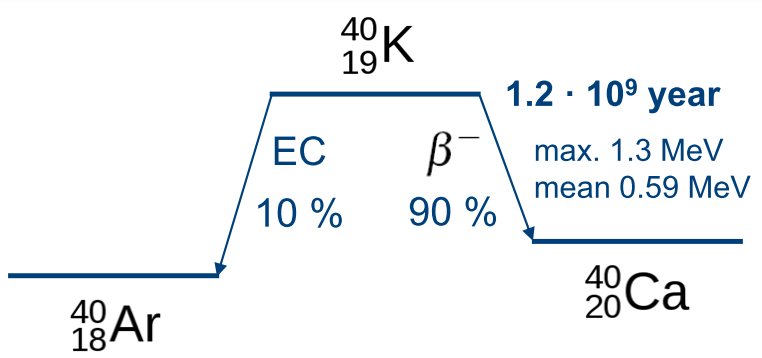
\includegraphics[width=0.5\textwidth]{figs/fig_40K_decay.png}
  \centering
  \caption{\label{fig:40Kdecay}
  \emph{Decay scheme of $^{40}$K.}}
\end{figure}

To compute the radiation dose due to $^{40}$K, we assume that this
dose is only due to the $\beta^-$ emission.  Suppose there are $N_0$
$^{40}$K atoms in a g at time $t = 0$. Then the number of radioactive
atoms at time $t$ equals
\begin{equation}
  N(t) = N_0 \; e^{- \ln 2 \frac{t}{T_{1/2}}}
\end{equation}
implying that the activity, i.e. the number of decaying atoms per unit of
time equals
\begin{equation}
  A(t) = - \frac{dN(t)}{dt} = \frac{\ln 2}{T_{1/2}} N(t).
\end{equation}
where we have to express $T_{1/2}$ in seconds to obtain a result in
Bq. Denoting the number of seconds per year as $s_y$, we have
$T_{1/2} = 1.25 \cdot 10^9 \; s_y$.

Avogadro's number equals $N_A = 6.022 \cdot 10^{23}$ atoms/mole, and 1 mole
of $^{40}K$ weighs 40 g. Consequently, the activity per kg tissue equals
\begin{equation}
  A = \frac{\ln 2}{T_{1/2}} \;
  \frac{N_A}{40 \mathrm{g}} \;
  \frac{2 \mathrm{g} \;}{\mathrm{kg}} \;
  \frac{1.2 \cdot 10^{-4} \,
    ^{40}\mathrm{K\_atoms}}{\mathrm{K\_atom}}
\end{equation}
This produces an activity per mass in Bq/kg.  In 90\% of these decays,
an electron is emitted which deposits on average an energy of 0.59
MeV. Thus, the energy deposited by a decay equals
\begin{equation}
  E = 0.9 \cdot 0.59 \cdot 10^6 \mbox{ eV} \cdot 1.6
    \cdot 10^{-19} \frac{\mbox{J}}{\mbox{eV}}
\end{equation}
Multiplying $A$ and $E$ produces the deposited energy per mass and per
s in J / (kg s) = Gy / s. Finally, we multiply this with the number of
seconds per year $s_y$ and with 1000 to obtain the result in mGy per
year:
\begin{align}
  &A\;E \; \frac{\mbox{1000 mGy}}{\mbox{Gy}} \frac{s_y}{\mbox{ year}}\\
  &= \frac{\ln 2}{1.25 \cdot 10^9 \; s_y} \;
  \frac{6.022 \cdot 10^{23}}{40} \;
  \frac{2 \cdot 1.2 \cdot 10^{-4}}{\mbox{kg}} \;
  0.9 \cdot 0.59 \cdot 10^6 \cdot 1.6 \cdot 10^{-19} \mbox{ J}
   \frac{\mbox{1000 mGy}}{\mbox{Gy}} \; \frac{s_y}{\mbox{ year}} \nonumber\\
  &= 0.17 \;\frac{\mbox{mGy}}{\mbox{year}}
\end{align}
This calculation seems OK, since the UNSCEAR 2008 report gives also
0.17 mSv for the effective dose from natural $^{40}$K irradiation.

\subsection{Thyroid therapy with $^{131}$I}
%=========================================
The thyroid has a strong affinity for iodine, and thyroid tumors
inherit this affinity from the normal cells. Consequently, a
beta-emitting isotope like $^{131}$I is a good radionuclide for
treating thyroid cancer. As can be seen in table
\ref{tab:rntisotopes}, $^{131}$I not only emits electrons, but also
several gammas. This has the drawback that the radionuclide trapped in
the tumor will not only irradiate the tumor with electrons, it will
also send some energy to the entire body as photons. But an advantage
of these photons is that they can be used for imaging with a gamma
camera or activity estimations with a gamma detector. Because several
of these gammas have high energies, imaging must be done with high
energy collimators, and detectors targeting the thyroid must be well
shielded to avoid contributions from $^{131}$I uptake in the rest of
the body.

To determine the activity to be administered, a low activity of
$^{131}$I is administered and imaging is performed to see which
fraction of the activity is taken up in the thyroid. For therapy
follow up, imaging (or photon counting) is be done to monitor the
$^{131}$I uptake in the thyroid as a function of time.

Figure \ref{fig:thyroid} illustrates the calibration and activity
monitoring with a photon counting detector (typically a NaI crystal
with PMT). A standard setup is used to scan the patient, to ensure
good reproducibility, such that after calibration the measurement is
quantitative. For calibration, a phantom mimicking the geometry and
attenuation of the neck is used, containing $^{131}$I at the position
of the thyroid.

\begin{figure}[htb]
  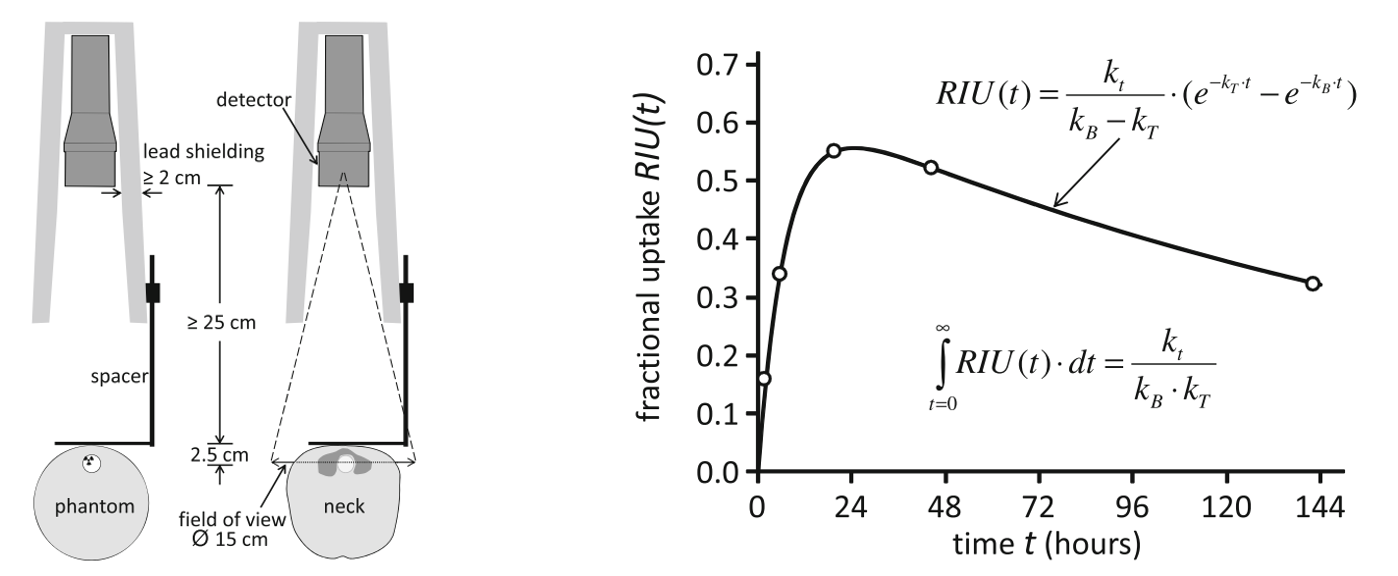
\includegraphics[width=0.95\textwidth]{figs/fig_thyroid_therapy.png}
  \centering
  \caption{\label{fig:thyroid} \emph{Thyroid therapy with
      $^{\it{131}}$I. At different time points, activity measurements are
      done with a simple detector, calibrated with a phantom. A tracer
      kinetic model is applied to estimate the time activity curve
      from a few measurements. The figures are from
      \cite{Haenscheid2013}. (RIU(t) denotes fractional $^{\it{131}}$I uptake
      in the target tissue at time t, and $k_t$, $k_B$ and $k_T$ are
      time constants of the kinetic model.)}}
\end{figure}

With this setup, the patient is scanned a few times over a week,
producing measurements of the activity in the thyroid. Then a kinetic
model is applied, to fit a smooth and realistic time-activity curve
through these points. A good model must be used, because estimating
the total dose to the thyroid involves a very strong extrapolation
beyond the last time point (see figure \ref{fig:thyroid}).


\subsection{$^{131}$I-mIBG therapy for neuroblastoma}
%==================================================
The compound mIBG (meta-iodobenzylguanidine) is taken up by cells of
the sympathetic nervous system. Neuroblastoma usually inherit this
affinity for mIBG, and as a result, $^{131}$I-mIBG can be used to
selectively irradiate these tumors. To circumvent the toxic effects on
the bone marrow (which makes red blood cells), stem cells are
collected before treatment and reinfused after the treatment. This
will ensure the production of blood cells after treatment. The
$^{131}$I-mIBG treatment is combined with Topotecan, a drug that makes
neuroblastoma more sensitive to radiation \cite{Gaze2015}.

The aim of the $^{131}$I-mIBG procedure, applied to treat children
with metastatic neuroblastoma, is to achieve a whole body dose of 4
Gy. It has been shown that with this whole body dose, the dose to the
neuroblastoma is sufficiently high and side effects are limited. To
achieve this, the therapy is given in two fractions. The first
fraction delivers a first whole body dose well below 4 Gy. In
addition, the photons emitted by $^{131}$I are used to determine the
whole body dose. This is often done with a simple gamma detector and
appropriate calibration, similar to what is shown in figure
\ref{fig:thyroid}, but this time focusing on the entire
body. Alternatively (and more accurately), planar imaging or SPECT can
be used. From that measured dose and the known amount of administered
activity in the first fraction, the amount of activity for the second
fraction is computed, to obtain the target dose of 4 Gy.

\begin{figure}[tb]
\centering
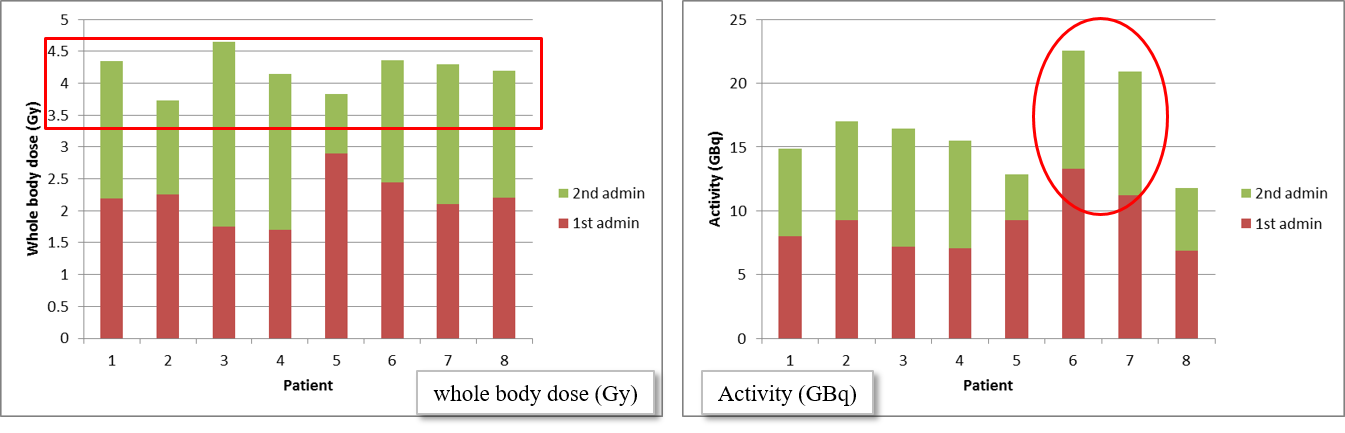
\includegraphics[width=\textwidth]{figs/fig_mIBG.png}
\caption{\label{fig:mibg} \emph{The whole body doses achieved in 8
    patients (left), and the activity that was administered to obtain
    this dose of approximately 4 Gy (right). The red and green blocks
    correspond to the first and second fraction, respectively. For
    patients 6 and 7, much more activity was needed to achieve the
    same whole body dose. Courtesy of Gaze et al. \cite{Sangro2012}.}}
\end{figure}
%
Figure \ref{fig:mibg} shows for 8 patients the whole body doses
produced by the two fractions. The dose of the first fraction was only
based on the patient weight, and produced roughly 2 Gy. This was used
to adjust the activity given in the second fraction, shown in the plot at
the right hand side in the figure. The plot at the left shows that
this produced a total dose of approximately 4 Gy. This treatment is
effective. However, more accurate tumor dose computation would be
useful, to provide more information about the relation between the
administered doses, the tumor control and the toxic effects to healthy
tissues, which would facilitate the development of even more effective,
personalized treatment.


\subsection{$^{90}$Y selective internal radiation therapy for liver tumors}
%============================================
The liver can be affected by a primary liver (hepatic) tumor or by
tumor metastases originating from elsewhere in the body.

One approach to treating liver tumors is radioembolization, i.e. to
release small radioactive spheres into the blood supplying the
tumors. These microspheres, made of resin or glass, have a diameter of
25-35 $\mu$m, which is small enough to travel through larger blood
vessels, and big enough to get stuck in the tumor
micro-vasculature. The microsphere then hinders or blocks the
perfusion through the microvessel, which is already bad for the
tumor. But more importantly, these microspheres contain a
$\beta$-emitting isotope. The emitted electrons interact with the
surrounding tissue, depositing their energy within a few mm from where
they are emitted. The aim is to have the microspheres accumulated in
or very close to the tumor lesions, such that the $\beta$-radiation
destroys the tumor with minimal damage to the healthy liver.

The liver is perfused not only by the hepatic artery, but also by the
portal vein. Veins are typically outputting blood from organs, but the
liver takes input from a vein too, because its task involves
processing venous blood from the stomach, intestines and
spleen. Healthy liver cells receive about 75\% of their blood from the
portal vein, and only 25\% from the hepatic artery. In contrast,
tumors take most of their blood from the hepatic artery. For that
reason, the microspheres are released via a catheter that is
maneuvered into the hepatic artery. To further increase selectivity,
the catheter is steered into one or a few branches of the hepatic
artery which are known to supply tumors. As illustrated in figure
\ref{fig:Sangro}, a better healthy tissue sparing can be achieved when
the tumor is more localized in the liver. For this reason, the
treatment is called {\em selective internal radiation therapy} (SIRT).
\begin{figure}[tb]
\centering
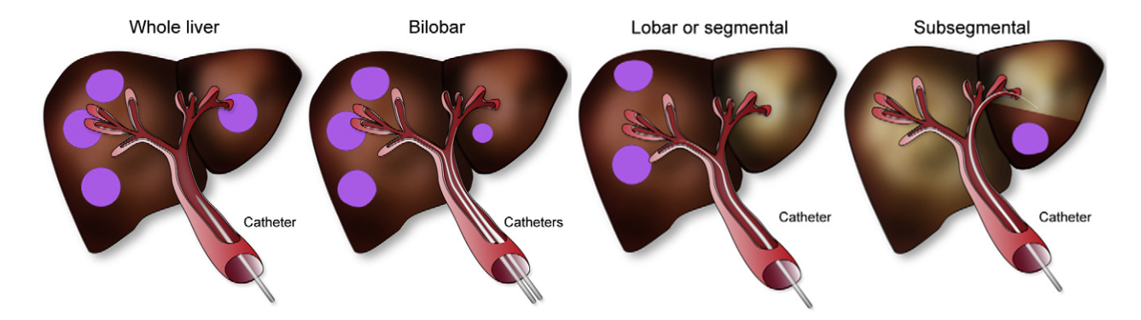
\includegraphics[width=0.9\textwidth]{figs/fig_SIRT_Sangro.png}
\caption{\label{fig:Sangro} \emph{Radioactive microspheres are sent
    into the liver through selected branches of the portal vein, targeting
    the tumors. \cite{Sangro2012}.}}
\end{figure}
One of the electron-emitting isotopes that is often used for SIRT
is the yttrium isotope $^{90}$Y. 

\subsubsection{Dose verification for SIRT with $^{90}$Y microspheres}
%'''''''''''''''''''''''''''''''''''''''''''''''''''''''''''''''''''
As shown in table \ref{tab:rntisotopes}, $^{90}$Y is really a pure
$\beta$-emitter, but in 32 of each million decays, it produces a
positron. Obviously, it is a poor positron emitter, but because the
treatment involves large doses (a few GBq), because the microspheres
are concentrated near the liver tumors and because the effective
sensitivity of current PET systems is high, it is possible to make
quantitative images of the $^{90}$Y distribution in the body of the
patient. Since the microspheres remain trapped for a long time in the
microvessels, we can assume that the microspheres concentrations
remain constant over time, and that the radioactive decay of $^{90}$Y
is the only cause of change to the activity concentration. Therefore,
we only need a single PET image for dose verification after
treatment. 

Since the electrons deposit their energy very close to their emission
source, the radiation dose to the tissues can be computed using the
``local deposition model''. That means that with good approximation,
the dose is proportional to the activity concentration achieved
shortly after injection: multiplication with a global scale factor
transforms the PET activity image with voxel values in Bq/ml to a
dose image with voxel values in Gy.

The time integrated activity $\tilde A$ equals
\begin{equation}
  \tilde A = \int_0^\infty A_0\; e^{- \frac{\ln 2}{T_{1/2}}} dt
  \;=\; A_0 \frac{T_{1/2}}{\ln 2}
\end{equation}
where $A_0$ is the activity in Bq in a particular region of interest,
and $T_{1/2}$ = 64.1 hours is the half life of $^{90}$Y. Following
equation (\ref{eq:mirddose}), the dose is obtained by multiplying
$\tilde A$ with the S-factor, given by equation (\ref{eq:Svalue}). For
$^{90}$Y, the S-factor reduces to
\begin{equation}
  S(r \leftarrow r) = \frac{E}{M(r)}
\end{equation}
where $M(r)$ is the mass of the region $r$ and $E$ is the average energy
of the emitted electron. Consequently, the accumulated dose in a
particular region $r$ equals
\begin{align}
  D_r &= S(r\leftarrow r) \; \tilde A\\
      &= \frac{A_0}{M(r)} \;E \;\frac{T_{1/2}}{\ln 2}\\
  &= \frac{A_0}{M(r)} \mbox{ 933.6 $\cdot 10^3$ eV } \cdot 1.6
     \cdot 10^{-19} \frac{\mbox{J}}{\mbox{eV}} \;
     \frac{\mbox{64.1 h} \cdot \mbox{3600 s/h}}{0.693}\\
  &= 49.7 \cdot 10^{-9} \;\mbox{Js} \; \frac{A_0}{M(r)}
\end{align}
Consequently, an activity of 1 GBq $^{90}$Y trapped in a region of 1
kg produces an accumulated radiation dose of approximately 50 Gy.

An image in Bq/ml can be converted to an image in Bq/g by dividing it
by the tissue density in g/ml, which is close to unity except for
bone and lung. An $^{90}$Y activity image in Bq/g can be converted to
accumulated dose in Gy, by multiplying it with
$49.7 \cdot 10^{-9}$ Js $\cdot$ 1000 g/kg = $49.7 \cdot 10^{-6}$ Gy\,g\,s.

% Annual exposure in Belgium (laatste dia van Kristof)

\subsubsection{SIRT treatment planning with \textsuperscript{99m}Tc\ labeled
  micro-aggregated albumin}
%''''''''''''''''''''''''''''''''''''''''''''''''''''
Albumin microaggregates (MAA) are very small particles (a few microns)
which tend to accumulate in microvasculature, much like resin or glass
microspheres. MAA labeled with \textsuperscript{99m}Tc\ are used to simulate a SIRT
treatment: the \textsuperscript{99m}Tc-MAA is released in selected branch(es) of
the portal vein, and the result is imaged with SPECT. SPECT imaging
must be done shortly after MAA-administration, because unlike the
therapeutic microspheres, MAA is only trapped temporally. The
\textsuperscript{99m}Tc-MAA study is done to check if the injected particles will
remain in the liver, or if a significant portion of them ends up in
the lungs. In some patients this happens, because their vasculature
has some liver-to-lung shunts. The study is also done to verify that
the catheterization procedure will reach all the tumors.  Figure
\ref{fig:SirtMaaY} shows transaxial slices from a pre-treatment
\textsuperscript{99m}Tc-MAA image and the corresponding post-treatment $^{90}$Y-PET
image. In this study, a good agreement between the pre- and
post-treatment images was obtained. 
%
\begin{figure}[h]
\centering
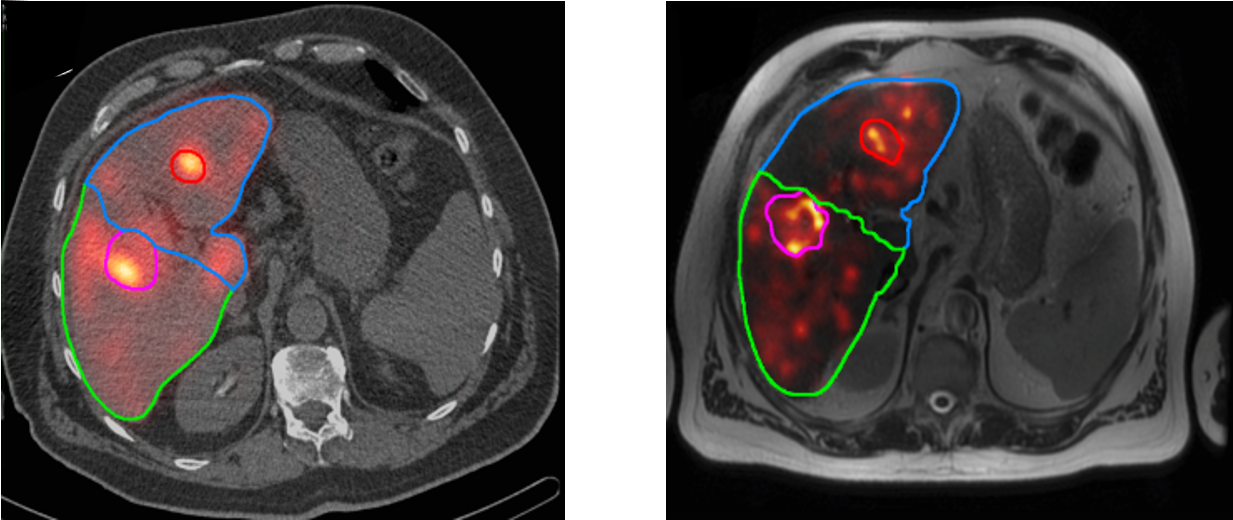
\includegraphics[width=0.9\textwidth]{figs/fig_SIRT_Tc_Y.png}
\caption{\label{fig:SirtMaaY} \emph{Left: the \textsuperscript{99m}Tc-MAA
    image (in color) fused with the corresponding CT image (black and
    white), from the pre-treatment SPECT/CT image. Right: the
    $^{90}$Y-PET image fused with the corresponding MR
    image, from the post-treatment PET/MR image.}}
\end{figure}
%

\section{Quantitative imaging}
%%%%%%%%%%%%%%%%%%%%%%%%%%%%%%
Treatment planning and dose verification require quantitative imaging,
since we need activity images in Bq/ml to compute dose images in
Gy. The creation and analysis of accurate dose images is not only
useful to verify if the treatment was successful, it also provides
valuable data to learn more about the complicated relationship between
radiation dose and biological effect, both in the tumors and the
normal tissues. This new knowledge should enable us to make
radionuclide therapy more effective. Doing that will require
more accurate treatment planning, and therefore also quantitative
imaging.\\[3mm]
%
As explained in previous chapters, PET and SPECT are quantitative,
provided that
\begin{itemize}
\item all corrections for sensitivity, attenuation, Compton
  scatter and/or randoms are performed well. 
\item the reconstructed image values are calibrated by determining the
  calibration factor, which converts the reconstructed voxel values
  into values in Bq/ml, see sections \ref{sec:spectquant} for SPECT
  and \ref{sec:scalefactor} for PET. The calibration factor is
  radionuclide dependent, and in particular in SPECT, this dependence
  is so complicated that it necessitates determining the calibration
  factor from phantom measurements for each tracer.
\end{itemize}



%\end{document}
